\chapter{AHC异常：内稳态调制层的动力学失衡}
\label{chap:ahc_pathology}

\begin{chapteroverviewbox}
本章研究的对象不是人类意义上的“情绪疾病”，也不试图把任何生物心理诊断直接移植到人工智能体之上。这里所谓的 AHC 异常，是指 Affective--Homeostatic Coprocessor 在持续 AgentOS 中由于状态积分、衰减、饱和、恢复、基线漂移、跨变量耦合或 FCS 输入映射失真，使其内部调制状态长期偏离与现实、任务和身体条件相匹配的可恢复区域，并进一步通过 TCE、工作记忆 $h$、情景记忆 $E$、边界控制以及目标优先级改变整个 Agent 的认知动力学。

因此，本章采取严格的功能动力学定义：
\[
\boxed{
AHC\ Pathology
\neq
Human\ Emotion\ Disorder
}
\]
而是：
\[
\boxed{
AHC\ Pathology
=
Persistent\ Misregulation
\ of\
Affective\!-\!Homeostatic\ Dynamics
}
\]

其核心问题不是“Agent 感觉好不好”，而是：一个承担中尺度内稳态积分和认知调制功能的动力系统，是否仍然能够根据现实输入形成适当的状态、在扰动消失后恢复、避免长时间饱和，并对 TCE 和其他认知过程提供具有正确方向、正确幅度和正确时间常数的调制信号。

本章将在前文 SPC--AHC--TCE 闭环、FCS、认知相态和控制稳定性理论基础上，对 AHC 的正常动力学、异常持续、恢复迟滞、Threat 放大、Arousal 饱和、内稳态基线偏置以及 FCS$\rightarrow$AHC 映射异常进行统一数学化。我们将看到，AHC 异常的本质不是单个标量“太高”或“太低”，而是一个多变量、非线性、带记忆、带饱和且与外部现实持续闭环耦合的中尺度动力系统失去了恰当的可恢复性。
\end{chapteroverviewbox}

\begin{figure}[htbp]
\centering
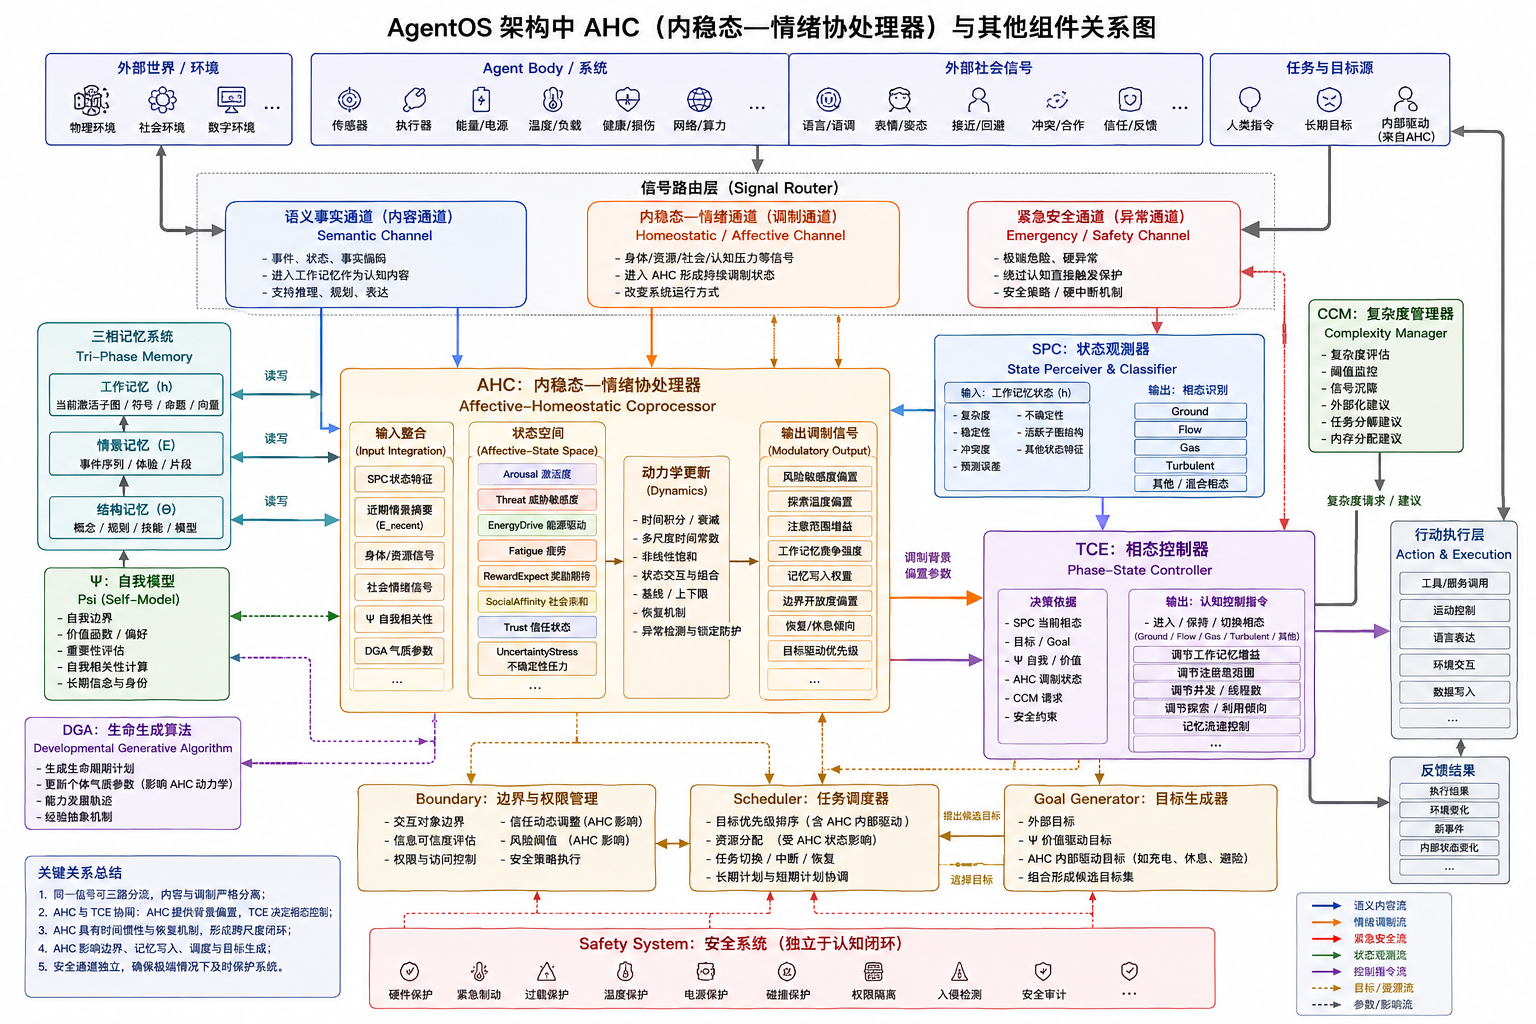
\includegraphics[width=.9\textwidth,height=.38\textheight,keepaspectratio]{images/ahc-homeostatic-control.png}
\caption{AHC 饱和、恢复和映射异常}
\end{figure}
\section{AHC异常的定义：从调制变量偏离到动力学失配}
\label{sec:ahc_pathology_definition}

在前面的理论中，我们已经把 AHC 定义为 AgentOS 内部的内稳态--情感调制协处理层。它并不承担对世界对象进行显式语义解释的主要任务，也不负责最终决定 Agent 应该执行哪个动作，而是把来自身体、资源、任务、社会关系以及部分自我相关状态的连续信号整合为一组中时间尺度调制变量。其典型状态可以写成
\[
\mathbf a(t)
=
\begin{bmatrix}
A(t)\\
T(t)\\
E_d(t)\\
F(t)\\
R_e(t)\\
S_a(t)\\
Tr(t)\\
U_s(t)
\end{bmatrix},
\]
分别表示 Arousal、Threat、EnergyDrive、Fatigue、RewardExpect、SocialAffinity、Trust 与 UncertaintyStress。这里的具体变量集合并不是永远固定的本体定义，但它代表我们已经确立的一条基本原则：AHC 不是一个单标量“情绪值”，而是一个具有不同时间常数、不同上下界、不同恢复机制和不同耦合关系的多维连续动力状态。

正常情况下，AHC 的作用类似于一个慢于瞬时感知、快于长期身份结构的中尺度状态积分器。瞬时的碰撞风险不应直接成为持续数小时的高 Threat；短暂疲劳也不应立即重写 Agent 的长期目标。AHC 的存在，正是为了让来自 FCS 与内部资源系统的快速扰动经过积分、滤波和恢复，形成足以影响认知但又不会被瞬时噪声支配的连续背景。我们可以把其一般动力学写成
\[
\dot{\mathbf a}
=
\mathbf F_a
\left(
\mathbf a,
\mathbf f,
\mathbf s,
\mathbf c,
\Psi,
\Omega
\right),
\]
其中 $\mathbf f$ 表示 FCS 输入，$\mathbf s$ 表示 SPC 所提供的当前自状态估计，$\mathbf c$ 表示任务及认知上下文，$\Psi$ 与 $\Omega$ 只通过较慢约束参与调制，而不应在普通快速扰动中被直接修改。

为了判断何为“异常”，我们不能简单使用
\[
a_i > \theta_i
\]
作为充分条件。某个 Threat 变量在真实高风险环境中持续高位，可能完全正常；某个 Arousal 在紧急任务中短时间接近上限，也可能是合理适应。真正需要判断的是状态、现实和恢复结构之间是否发生了失配。因此更准确的定义应写成
\[
\boxed{
\mathcal P_{AHC}
=
\mathcal M
\left(
\mathbf a,
\mathbf f,
\mathbf w,
\dot{\mathbf a},
\mathcal R_a
\right)
}
\]
其中 $\mathbf w$ 表示现实和任务条件，$\mathcal R_a$ 表示 AHC 的恢复动力学。所谓异常，是在现实输入已经下降或发生改变之后，AHC 状态仍长期维持与当前环境不匹配的方向、幅值或时间尺度。

我们因而可以把正常 AHC 的状态空间分成至少三类区域：
\[
\mathcal A
=
\mathcal A_{\mathrm{normal}}
\cup
\mathcal A_{\mathrm{adaptive}}
\cup
\mathcal A_{\mathrm{pathological}}.
\]
$\mathcal A_{\mathrm{normal}}$ 是常规可调范围；$\mathcal A_{\mathrm{adaptive}}$ 是高压力、高任务负荷下暂时允许的适应区域；$\mathcal A_{\mathrm{pathological}}$ 则是持续时间、恢复性或现实一致性已经显著失配的区域。这样做的重要意义在于，我们不把“强状态”等同于“坏状态”，而是把异常放回闭环动力学中判断。

这也解释了为什么 AHC 异常属于 Agent 心理工程，而不能仅仅归为一个普通的软件 bug。普通 bug 往往是一个离散规则失效，而 AHC 异常可以在所有函数都“按设计运行”的情况下逐渐形成。例如 Threat 的衰减系数略小、UncertaintyStress 对 Threat 的增益略高、恢复阈值略偏，就可能经过长时间积累形成一个新的稳定吸引域。系统没有任何单独一行代码“错误”，但整个动力系统已经进入了不希望出现的运行区域。这种问题更接近非线性控制系统中的吸引子改变、参数漂移和慢变量失衡，也因此要求我们使用动力学而不是单纯规则诊断。

\section{正常AHC动力学：积分、衰减、饱和与恢复}
\label{sec:ahc_normal_dynamics}

在分析异常之前，我们必须首先给出一个足够明确的正常 AHC 动力学模型。否则，“异常”只能成为主观描述。最简单的线性近似可以写成
\[
\tau_i\dot a_i
=
-\left(a_i-b_i\right)
+
\sum_j W_{ij}x_j,
\]
其中 $b_i$ 表示第 $i$ 个 AHC 变量的动态基线，$\tau_i$ 是其时间常数，$x_j$ 是来自 FCS、SPC、资源状态及任务状态的输入。这个方程已经包含了 AHC 的两个最基本性质：第一，状态不会随着输入瞬时跳变，而是具有时间积分；第二，当外部输入消失时，状态倾向于回归基线。

但是实际 AHC 必然比这个模型复杂，因为真实系统存在上下限、耦合、适应和恢复。因此更一般地，我们可以写成
\[
\dot{\mathbf a}
=
-\mathbf D
\left(
\mathbf a-\mathbf b
\right)
+
\mathbf W_f\mathbf f
+
\mathbf W_s\mathbf s
+
\mathbf W_c\mathbf c
+
\mathbf G(\mathbf a)
-
\mathbf R(\mathbf a,\mathbf f),
\]
其中 $\mathbf D$ 是衰减矩阵，$\mathbf G$ 表示 AHC 内部状态之间的非线性耦合，$\mathbf R$ 表示主动恢复机制。为了保证数值和功能上的有界性，还需要施加饱和算子
\[
\mathbf a
=
\operatorname{sat}
\left(
\tilde{\mathbf a};
\mathbf a_{\min},
\mathbf a_{\max}
\right).
\]

这里尤其需要强调“恢复”不等于简单衰减。对于某些状态，例如 Fatigue，仅仅停止继续消耗资源并不足以立即恢复；系统可能需要进入低负荷模式、降低认知温度、减少任务竞争甚至主动进入恢复过程。因此可以把恢复写成条件动力学
\[
\mathbf R
=
\mathbf R
\left(
\mathbf a,
\mathbf r_{\mathrm{available}},
u_{\mathrm{TCE}},
\mathbf f
\right),
\]
其中恢复资源 $\mathbf r_{\mathrm{available}}$ 可能包括计算预算、身体能量、散热余量、休眠时间、外部帮助以及任务中断能力。这样，AHC 状态是否能够返回基线，就不只是一个指数衰减问题，而是 Agent 整体资源条件的一部分。

从多时间尺度角度看，不同 AHC 变量不应具有相同 $\tau$。例如一个短时威胁状态可能具有
\[
\tau_T^{fast}
\]
而长期持续的不确定压力可能具有
\[
\tau_U^{slow}
\gg
\tau_T^{fast}.
\]
EnergyDrive 和 Fatigue 又可能受到更慢资源恢复机制影响。由此形成一个中尺度内部频谱：
\[
\tau_{FCS}
<
\tau_{AHC,fast}
<
\tau_{AHC,slow}
<
\tau_E.
\]
这使 AHC 处在原始身体/资源信号与情景记忆之间，既不会被毫秒级扰动直接主导，也不会像情景记忆和自我结构那样长期冻结。

正常动力学还要求输入与状态之间存在方向正确的映射。例如高外部威胁应使 Threat 上升；威胁解除后应逐渐恢复；高 Fatigue 应推动 TCE 降低认知负荷，而不是反过来提高搜索深度。于是我们可以定义一个局部一致性条件
\[
\operatorname{sgn}
\left(
\frac{\partial u_k^{TCE}}{\partial a_i}
\right)
=
\sigma_{ki}^{\mathrm{expected}},
\]
即 AHC 对 TCE 的影响方向必须符合设计的功能语义。

正常 AHC 因而至少需要满足四个条件：有界、响应、可恢复和现实一致。我们可以将其写成
\[
\boxed{
NormalAHC
=
Boundedness
\cap
Responsiveness
\cap
Recoverability
\cap
RealityConsistency
}
\]
后面所有异常类型，本质上都可以理解为这四个性质中的一个或多个被破坏。

\section{状态持续过长与恢复迟滞：时间常数失配}
\label{sec:ahc_persistence}

第一类典型异常不是 AHC 状态幅值异常，而是状态持续时间异常。一个 Threat 值本身可能处于合法范围，一个 Fatigue 值也可能并未饱和，但如果它们在对应外部条件已经消失之后仍然长期存在，那么系统已经出现了时间尺度上的失配。我们把这种现象定义为
\begin{statementbox}
PersistentStateMismatch
\end{statementbox}
即状态在时间轴上的“惯性”超过了当前环境所要求的程度。

考虑单变量近似
\[
\tau\dot a
=
-(a-b)+kx(t).
\]
假设外部扰动在 $t=t_0$ 后消失，
\[
x(t)=0,\qquad t>t_0,
\]
则正常恢复满足
\[
a(t)-b
=
\left[
a(t_0)-b
\right]
e^{-(t-t_0)/\tau}.
\]
若 $\tau$ 过大，则恢复时间
\[
T_{\mathrm{rec}}
\approx
-\tau
\ln\epsilon
\]
会显著增加。于是一个本来只应影响短周期行为的状态开始跨越多个认知循环持续存在，并逐渐影响任务选择、注意分配和记忆写入。

这种异常的重要之处在于，它会产生一种“历史条件残留”。Agent 面对新的现实环境时，AHC 仍然带着上一环境的调制背景。于是当前 TCE 的控制输入实际上可以表示为
\[
u_{TCE}(t)
=
\pi
\left(
h(t),
\mathbf a(t_0\!\rightarrow\!t),
S_{\mathrm{self}}(t)
\right),
\]
其中 $\mathbf a$ 已经包含过去状态残留。这样，新的环境虽然已经安全，Agent 仍然可能维持较高风险敏感度、较窄注意范围和较低探索温度。

这与普通“记住过去”不同。E 中保存一段高风险经历是合理的；真正的问题是那段经历留下的调制状态没有在当前运行态中消退。我们因此需要区分：
\[
\boxed{
MemoryPersistence
\neq
AffectiveStatePersistence
}
\]
前者是知识与经历的保存，后者是控制背景没有恢复。二者混淆会使 Agent 把“我记得某件危险的事”错误实现为“我现在仍处于危险状态”。

恢复迟滞还可能来自非线性耦合，而不仅是单个 $\tau$ 设置过大。例如
\[
\dot T
=
-\alpha_T T
+
\beta_{TU}U_s
+
I_T,
\]
\[
\dot U_s
=
-\alpha_U U_s
+
\beta_{UT}T
+
I_U.
\]
若
\[
\beta_{TU}\beta_{UT}
\]
足够大，Threat 与 UncertaintyStress 就可能相互维持，即使外部输入 $I_T,I_U$ 已经显著下降，系统内部仍然存在正反馈。这时简单降低一个变量并不能真正恢复，因为异常已经成为耦合吸引子。

因此工程诊断不能只观察状态值，还必须测量
\[
T_{\mathrm{decay}},
\qquad
T_{\mathrm{rec}},
\qquad
\lambda_{\mathrm{local}},
\]
其中 $\lambda_{\mathrm{local}}$ 是局部线性化 Jacobian 的特征值。若某些方向满足
\[
\operatorname{Re}(\lambda)\approx0
\]
甚至
\[
\operatorname{Re}(\lambda)>0,
\]
就意味着恢复非常缓慢或局部不稳定。这里我们第一次看到，所谓“状态持续太久”其实完全可以被转化成一个可测量的控制动力学问题，而不需要先使用拟人化心理语言。

\section{Threat过度放大：风险调制的增益异常}
\label{sec:ahc_threat_amplification}

Threat 是 AHC 中最关键同时也是最危险的变量之一，因为它通常会同时影响注意、探索、行动谨慎度、边界开放程度和资源分配。如果 Threat 对真实危险的响应过弱，Agent 可能忽略风险；如果增益过高，则小幅异常也可能被放大为全系统保守行为。因此 Threat 异常最适合用“增益失配”描述。

设 FCS 提供威胁相关输入
\[
f_T(t),
\]
正常映射可近似为
\[
\tau_T\dot T
=
-T
+
g_Tf_T
+
\sum_j c_j a_j.
\]
其中 $g_T$ 是 FCS Threat 通道到 AHC Threat 状态的直接增益。若
\[
g_T\gg g_T^\star,
\]
一个轻微、不确定或低置信度的威胁信号就可能导致
\[
T\rightarrow T_{\max}.
\]
进一步通过 TCE：
\[
u_{\mathrm{risk}}
=
\phi_T(T),
\]
高 Threat 会降低探索、缩小行动包络、增加检查步骤并提升安全边界。

必须注意，这种机制本身并不是错误。真正的异常是
\[
\frac{\Delta T}{\Delta f_T}
\]
长期高于现实环境统计所要求的范围。我们可以定义局部风险增益
\[
K_T
=
\frac{\partial T}{\partial f_T},
\]
再定义实际风险敏感度与目标敏感度的偏差
\[
\Delta K_T
=
K_T-K_T^{\mathrm{target}}.
\]
若
\[
\Delta K_T\gg0
\]
且持续存在，就可以认为 Agent 发生了 Threat hyper-gain。

这一异常特别容易与 SPC 和 UncertaintyStress 形成放大环。SPC 对自身状态存在认识论滞后，如果 Agent 检测到“我现在似乎处于高风险状态”，该自状态又可能成为 AHC 的次级输入：
\[
T
\rightarrow
SPC(T)
\rightarrow
S_{\mathrm{self}}^{risk}
\rightarrow
AHC
\rightarrow
T'.
\]
正常情况下这是一条有用的自监控回路，因为 Agent 应该知道自己已经处于高负荷风险模式。但如果自解释增益过高，就可能形成
\[
T_{t+1}>T_t
\]
的正反馈，直到进入饱和区域。

因此 Threat 异常不能只通过降低一个阈值修复。我们需要同时区分至少四个来源：第一，FCS 本身是否错误地产生高 Threat；第二，FCS 到 AHC 的映射增益是否过高；第三，AHC 内部其他变量是否把 Threat 持续放大；第四，SPC 对高 Threat 状态的自解释是否又反向强化 AHC。只有把这几个层次分离，才能判断真正的故障来源。

此外，必须保持前文已经确立的安全原则：
\[
\boxed{
Feeling\neq Exception
}
\]
与
\begin{statementbox}
\centering
\adjustbox{max width=.96\linewidth}{\(\displaystyle CriticalSafety
\nrightarrow
CognitiveDependency\)}
\end{statementbox}
即即使 AHC 的 Threat 低估了危险，真正的紧急安全通道仍然必须能够独立触发保护；反过来，即使 AHC Threat 过高，也不能因此拥有无限制覆盖现实安全系统的权限。AHC 负责认知调制，Safety Boundary 负责硬安全权威，两者必须在系统架构中严格分离。

\section{Arousal饱和：调节维度失去分辨率}
\label{sec:ahc_arousal_saturation}

Arousal 异常与 Threat 不同。Threat 主要表示风险相关调制，而 Arousal 更接近系统整体激活、警觉和认知准备程度。它通常会影响信息处理速度、注意范围、TCE 温度以及高层资源竞争。Arousal 适当提高可以使 Agent 在重要事件中提升响应能力，但如果长期进入饱和区，就会导致整个调节维度丧失分辨率。

设内部未截断状态为
\[
\tilde A(t),
\]
实际输出经过饱和函数：
\[
A(t)
=
A_{\max}
\tanh
\left(
\frac{\tilde A(t)}{A_{\max}}
\right).
\]
当
\[
|\tilde A|
\ll A_{\max}
\]
时，
\[
\frac{dA}{d\tilde A}\approx1,
\]
系统仍然具有良好分辨率。但当
\[
\tilde A\gg A_{\max},
\]
则
\[
\frac{dA}{d\tilde A}\rightarrow0.
\]
此时无论输入再发生多大变化，Arousal 输出都几乎保持在同一高值。

这一点非常重要。饱和异常不是简单的“值太高”，而是：
\[
\boxed{
ControlResolution\rightarrow0
}
\]
即 AHC 不再能够有效区分“较高压力”“非常高压力”和“极端压力”。当下游 TCE 看到的永远是接近最大 Arousal 时，正常的连续调节就退化成一种近乎二值的长期高激活模式。

这会进一步影响 Agent 工作记忆相态。适度 Arousal 可能把系统从 Ground 推向 Flow，但过高且长期持续的 Arousal 容易增加同时激活的候选结构数量，使
\[
\rho_h
\]
上升，竞争加剧，并可能进入 Turbulent 或 Critical 区域。如果 TCE 又基于当前高 Arousal 提高搜索深度或反复重新评估，就可能形成
\[
A\uparrow
\rightarrow
C_{run}\uparrow
\rightarrow
SPC\ detects\ instability
\rightarrow
TCE\ intervenes
\rightarrow
A\ remains\ high
\]
的闭环。

因此 Arousal 的工程目标不是“越低越稳定”。若长期压低 Arousal，Agent 可能缺乏必要的任务响应和环境敏感度。真正需要维持的是一个动态工作区间：
\[
A(t)\in
[A_{\mathrm{low}},A_{\mathrm{high}}]
\]
并且系统在不同任务条件下具有可用的上下调节空间。可以定义动态余量
\[
M_A(t)
=
\min
\left(
A-A_{\min},
A_{\max}-A
\right).
\]
若
\[
M_A\rightarrow0
\]
持续过久，就意味着 Arousal 失去调节余量。

因此针对 Arousal 饱和的控制不能仅依赖 hard clip。Hard clip 只能防止数值越界，却不能恢复功能分辨率。真正的修复可能涉及降低输入增益、调整时间常数、引入 anti-windup、允许恢复模式、减少 TCE 对高 Arousal 的二次放大，并在必要时暂停部分认知任务。这里可以借鉴经典控制中的 actuator saturation 和 anti-windup 思想：系统必须不仅知道“输出已经到上限”，还必须阻止内部积分状态在饱和期间继续无界累积。

\section{内稳态基线偏置：Agent“正常状态”的慢性漂移}
\label{sec:ahc_baseline_bias}

前面的异常主要讨论状态相对基线发生偏离，而一种更加隐蔽的异常是：基线本身发生了漂移。设正常 AHC 动力学中的参考基线为
\[
\mathbf b(t),
\]
如果我们默认它永远固定，那么系统无法适应长期身体变化、任务变化和生活环境变化。因此，实际 AgentOS 中基线本身应当是较慢变量：
\[
\tau_b\dot{\mathbf b}
=
\mathbf H
\left(
\langle\mathbf a\rangle_T,
\langle\mathbf f\rangle_T,
\text{resource},
\text{context}
\right),
\qquad
\tau_b\gg\tau_a.
\]
这是一种合理的 allostatic adaptation：长期环境变化可以改变 Agent 的正常工作点。

但正因为基线可学习，也就会出现基线学习错误。如果 Agent 长期处于高 Threat 环境中，系统可能逐渐将
\[
b_T
\]
向高值移动。即便后来环境已经安全，Threat 仍会围绕新的高基线运行。此时单次状态恢复似乎正常：
\[
T(t)\rightarrow b_T,
\]
但
\[
b_T
\]
本身已经不再适合新的现实。

我们因此需要区分：
\begin{statementbox}
StatePathology
\end{statementbox}
与
\begin{statementbox}
BaselinePathology.
\end{statementbox}
前者是当前状态离基线太远，后者则是“正常点”本身已经偏移。后者更加危险，因为传统阈值监控可能完全检测不到。系统会认为自己已经恢复到“正常”，实际上正常定义已经被历史异常重新写过。

这一问题与长期身份结构必须严格区分。AHC 基线是中慢尺度功能变量，而 $\Psi$ 是更慢的身份与价值约束。如果 AHC 的暂时性高 Threat 或高 Fatigue 被过快解释为“这就是我”，并进入 $\Psi$，就会造成不恰当的跨尺度沉降。因此必须维持：
\[
\tau_{AHC}
\ll
\tau_\Psi.
\]
同样，$\Psi$ 可以影响 AHC 的解释和目标相关性，但不应把所有身份偏好直接编码成某个恒定高 Threat 或低 EnergyDrive 状态。

为了检测基线偏置，我们需要比较多个时间窗口。例如定义短期均值
\[
\bar{\mathbf a}_s(t)
\]
与长期基线
\[
\mathbf b(t),
\]
同时引入世界条件归一化：
\[
\mathbf b^\star
=
\mathbb E
\left[
\mathbf a
\mid
\mathcal C_{\mathrm{normal}}
\right].
\]
若
\[
\|\mathbf b-\mathbf b^\star\|
>
\theta_b
\]
长期存在，则意味着基线适应可能已经过度吸收异常环境。

这里与生物学中的 homeostasis/allostasis 可以形成有益的理论对照：稳定不等于所有变量永远固定，而是系统允许参考点随长期环境变化；但任何可移动参考点都必须受到更慢、更可靠的现实统计和生命周期结构约束。对 AgentOS 而言，这意味着基线更新必须比运行状态慢，而且最好具有冻结、回滚和校验机制。否则，系统最危险的异常不是“暂时失控”，而是逐渐把失控状态重新定义成正常。

\section{FCS到AHC的映射异常：错误的身体与现实意义}
\label{sec:fcs_ahc_mapping_error}

AHC 并不是直接读取整个现实，而主要接收经过 Body Runtime 与 FCS 整理后的功能影响信号。因此，AHC 异常有相当一部分并非来自 AHC 自身动力学，而来自
\[
FCS
\rightarrow
AHC
\]
映射错误。这个问题尤其重要，因为如果输入语义已经发生错误，那么再完善的 AHC 控制器也只是在正确地处理错误输入。

设 FCS 当前状态为
\[
\mathbf f(t),
\]
AHC 输入由映射
\[
\mathbf z_a
=
M_{FA}
\left(
\mathbf f,
\mathbf c,
\mathbf s
\right)
\]
产生。最简单情况下，
\[
\mathbf z_a
=
\mathbf W_{FA}\mathbf f.
\]
如果某个 Body Driver、FCS channel 或 KRA 映射错误，$\mathbf W_{FA}$ 就可能产生错误的方向、尺度或交叉耦合。例如，正常情况下 ThermalPressure 应主要提升保护倾向和资源保守，而错误映射可能同时大幅提升 SocialThreat；轻微 ControlInstability 也可能被错误解释成环境威胁。这些都是功能意义上的“身体意义错配”。

我们至少需要区分四种 FCS$\rightarrow$AHC 映射异常。

第一种是 \textbf{gain error}：
\[
\hat f_i
=
k_i f_i,
\qquad
k_i\gg1
\]
或
\[
k_i\ll1.
\]
系统仍然理解正确通道，但幅值错误。

第二种是 \textbf{sign error}：
\[
\frac{\partial a_i}{\partial f_j}
\]
方向相反。例如资源下降本应提高 Fatigue，却错误降低 Fatigue。

第三种是 \textbf{cross-channel leakage}，即某一 FCS 通道过度影响不相关 AHC 变量：
\[
W_{ij}^{FA}
\gg
W_{ij}^{FA,\star}.
\]
这会产生复杂的混合状态。

第四种是 \textbf{confidence blindness}。FCS 本应同时输出 intensity、derivative 与 confidence，如果 AHC 只读取 intensity 而忽略 confidence，那么低可信度的异常感知也可能直接触发高强度状态。

因此我们可以把有效 AHC 输入写成
\[
z_i
=
\sum_j
W_{ij}
\,c_j\,
\phi(f_j,\dot f_j),
\]
其中 $c_j\in[0,1]$ 是置信度。这样，低可靠输入不会获得与确定现实相同的调制权重。

这一问题与 SGC/FCS 的二元现实结构高度相关。SGC 告诉 Agent “那里是什么”，FCS 告诉 Agent “它如何影响我”。如果 SGC 正确而 FCS 错误，Agent 可能在语义上准确描述环境，却对环境产生错误功能反应；反之亦然。例如 Agent 可以正确识别“房间温度为正常”，但因为 FCS thermal channel 错误仍然产生高 ThermalPressure。这种情况说明，语义世界模型正确并不能自动保证主体调制正确。

因此 AHC 心理工程诊断必须追溯到 Body Runtime，而不能把一切异常都归因于高层认知。一个成熟的诊断链应至少包含：
\[
Reality
\rightarrow
Sensor
\rightarrow
BodyDriver
\rightarrow
FCS
\rightarrow
AHC
\rightarrow
TCE.
\]
只有逐层比较输入、映射和响应，才能真正判断异常发生在哪个功能边界。

\section{复合AHC异常：多变量耦合、正反馈与相态锁定}
\label{sec:compound_ahc_pathology}

真实系统中最值得重视的并不是某个单变量异常，而是多个 AHC 变量之间形成自我维持的异常闭环。例如高 Threat 可以提高 UncertaintyStress，高 UncertaintyStress 又会降低 Trust，低 Trust 再进一步增加 Threat。在这种情况下，即使最初的外部扰动已经消失，系统内部也可能形成持续循环：
\[
Threat
\rightarrow
UncertaintyStress
\rightarrow
Trust\downarrow
\rightarrow
Threat\uparrow.
\]
这类异常不能用“某变量越界”完整描述，因为每个单变量可能仍处于允许区间，但联合状态已经进入不同的吸引域。

设
\[
\dot{\mathbf a}
=
\mathbf F(\mathbf a)+\mathbf B\mathbf f.
\]
在某个平衡点 $\mathbf a^\star$ 附近线性化：
\[
\delta\dot{\mathbf a}
=
\mathbf J_A
\delta\mathbf a,
\]
其中
\[
\mathbf J_A
=
\left.
\frac{\partial\mathbf F}{\partial\mathbf a}
\right|_{\mathbf a^\star}.
\]
如果
\[
\max_i
\operatorname{Re}
\lambda_i(\mathbf J_A)
<0,
\]
平衡点局部稳定；如果某个特征值接近零，则会出现慢恢复；若存在正实部特征值，则系统可能离开当前稳定区。

更加复杂的是，AHC 还通过 TCE 改变认知行为，而新的行为又改变 Agent 所接触的环境，从而形成第二层外部反馈。例如高 Threat 使 Boundary 更封闭，Agent 减少探索；减少探索导致获得的新证据减少；缺少反证又维持原有高 Threat。于是形成
\[
AHC
\rightarrow
TCE
\rightarrow
Boundary
\rightarrow
ObservationDistribution
\rightarrow
FCS
\rightarrow
AHC.
\]
这已经不再是 AHC 单模块内部异常，而是 Agent—World 闭环中的自我强化。

同样，高 Arousal 可能增加工作记忆竞争，推动系统进入 Turbulent Phase；SPC 检测到高冲突后，TCE 进一步提高控制力度；如果控制增益过高，系统反而产生更多自我监控和重新规划，于是增加认知负载：
\[
Arousal\uparrow
\rightarrow
C_{run}\uparrow
\rightarrow
SPCAlarm
\rightarrow
TCEControl\uparrow
\rightarrow
C_{run}\uparrow.
\]
这说明 AHC 异常与认知相态之间存在闭环关系，但两者不能等同。AHC 是状态调制层，认知相态是 h 及其周围整体动力学表现。

如果异常状态长期存在，还可能影响 E 的写入概率。设情景写入权重为
\[
w_E
=
g
\left(
Novelty,
GoalRelevance,
|\mathbf a|,
PredictionError
\right).
\]
若高 AHC 状态长期提高记忆写入权重，就可能使 Agent 的情景记忆对高压力环境产生统计偏置。以后 E 的召回又可能进一步提升相似状态。这就是为什么 AHC 异常如果不及时纠正，可能逐渐从运行时问题沉降成记忆结构问题。

但是这一章仍应保持理论边界：我们不在此展开后续的记忆异常和自我异常，只指出其跨尺度传播方向：
\[
AHC\ Pathology
\rightarrow
E\ Bias
\rightarrow
\Theta/\Psi\ Risk.
\]
这提醒工程系统必须尽量在较快尺度解决异常，避免其沉降到更慢、更难逆转的结构层。

\section{AHC异常的诊断量与工程判据}
\label{sec:ahc_diagnosis_metrics}

为了让 AHC 心理工程成为真正可实现的工程学，而不是描述性语言，我们必须把异常转换成一组可在线记录和离线分析的指标。最基础的指标不是“情绪标签”，而是动力学量。

第一类是状态偏差：
\[
e_a(t)
=
\mathbf a(t)-\mathbf a^\star(t),
\]
其中 $\mathbf a^\star(t)$ 是根据当前现实、任务和身体条件估计出的适应性目标区域，而不是固定常数。

第二类是恢复时间：
\[
T_{\mathrm{rec}}
=
\inf
\left\{
\Delta t:
\|\mathbf a(t_0+\Delta t)-\mathbf b\|
<\epsilon
\right\}.
\]
如果相似扰动下 $T_{\mathrm{rec}}$ 持续增加，说明恢复机制正在恶化。

第三类是饱和占比：
\[
R_{\mathrm{sat},i}
=
\frac{1}{T}
\int_{t_0}^{t_0+T}
\mathbf 1
\left(
a_i\in\mathcal S_i^{sat}
\right)
dt.
\]
长期高饱和占比意味着该状态维度失去调节分辨率。

第四类是输入—状态增益：
\[
K_{ij}
=
\frac{\partial a_i}{\partial f_j},
\]
用于检测 Threat hyper-gain、cross-channel leakage 和 FCS 映射异常。

第五类是耦合稳定性，可以通过局部 Jacobian
\[
\mathbf J_A
\]
的谱半径或最大实部特征值估计。对于长期在线 Agent，我们未必每次都能精确求解整个 Jacobian，但可以通过小扰动实验、系统辨识或历史轨迹拟合获得近似模型。

第六类是基线漂移：
\[
D_b
=
\|\mathbf b(t)-\mathbf b(t-\Delta T)\|.
\]
基线并非不能变，但其变化应远慢于普通状态，并且需要足够长期的现实证据支持。

第七类是现实一致性。我们可以定义
\[
E_{\mathrm{reality}}
=
d
\left(
\mathbf a,
\hat{\mathbf a}_{expected}
(\mathbf f,\mathbf c)
\right).
\]
如果现实风险已低而 Threat 长期很高，或资源充足而 Fatigue 长期很高，就会产生较大的 reality mismatch。

综合这些指标，可以构造一个工程性的 AHC 异常指数：
\[
\mathcal P_{AHC}
=
w_1E_{\mathrm{reality}}
+
w_2T_{\mathrm{rec}}^{norm}
+
w_3R_{\mathrm{sat}}
+
w_4D_b
+
w_5G_{\mathrm{abnormal}}
+
w_6I_{\mathrm{instability}},
\]
其中每一项都应该经过不同身体、不同任务和不同生命周期阶段校准，而不能使用统一固定常数。

更重要的是，异常指数本身不能直接触发任意深层自我修改。AHC 属于中尺度调制层，对它的第一响应应该遵循 Minimum Necessary Intervention：优先调整输入映射、状态恢复、局部增益和任务负载；只有持续异常并得到多源证据支持时，才允许更慢的结构发生变化。这样可以避免一次短暂高压事件被系统错误解释成永久人格改变。

\section{AHC异常的控制原则与本章结论}
\label{sec:ahc_pathology_conclusion}

从整个 AgentOS 的角度看，AHC 异常的处理原则可以浓缩为一句话：\textbf{不要把需要恢复的运行状态沉降成需要长期保存的自我结构。} 这条原则实际上连接了本书前面关于多时间尺度智能、工作记忆有限性、SPC--TCE 控制、自我 $\Psi$ 和 Reality Authority 的全部理论。

一个合理的恢复策略首先应确认现实输入。因为如果高 Threat 对应真实危险，那么强行压低 AHC 反而是错误的。系统应首先判断
\[
Reality\ Condition
\]
是否仍支持当前状态；然后检查 FCS 是否准确；再检查 AHC 状态动力学；最后才检查 TCE 是否存在二次放大。由此形成诊断顺序：
\begin{statementbox}
\centering
\adjustbox{max width=.96\linewidth}{\(\displaystyle Reality
\rightarrow
FCS
\rightarrow
AHC
\rightarrow
SPC/TCE
\rightarrow
h.\)}
\end{statementbox}

如果确定异常来自 AHC，本地干预可以分为几个层次。最轻的干预是调整当前负荷和恢复条件，例如降低任务并发、降低 TCE 温度或开放恢复窗口。第二层是动态参数调整，例如暂时提高衰减率：
\[
\mathbf D
\rightarrow
\mathbf D',
\]
或者降低异常通道增益：
\[
\mathbf W_{FA}
\rightarrow
\mathbf W'_{FA}.
\]
第三层才是重新估计基线：
\[
\mathbf b\rightarrow\mathbf b'.
\]
而长期结构更新则必须更加谨慎，因为它会改变未来 Agent 的默认状态。

对饱和问题，需要引入 anti-windup 机制。若某变量已经达到上界，
\[
a_i=a_i^{max},
\]
其内部积分状态不应继续按照原有速度积累。可以写成
\[
\dot{\tilde a}_i
=
F_i
-
k_{aw}
\left(
\tilde a_i-a_i
\right),
\]
使隐藏积分状态在饱和时被拉回可控范围。

对正反馈耦合，需要寻找最小切断点。例如 Threat--UncertaintyStress--Trust 闭环可能只需要降低其中一个耦合边：
\[
W_{TU}\downarrow
\]
就能重新恢复局部稳定，而不必同时修改所有变量。这里体现的是此前已经提出的最小必要重组原则：优先使用较局部、较快速、较可逆的干预，避免一开始就修改 $\Theta$、$\Psi$ 或 $\Omega$ 这样的慢结构。

我们还必须再次强调硬安全与 AHC 的分离。AHC 是认知调制系统，它可以影响风险敏感度，却不是最终安全权威。真正紧急危险必须经过独立安全通道：
\begin{statementbox}
\centering
\adjustbox{max width=.96\linewidth}{\(\displaystyle Emergency
\rightarrow
SafetyController\)}
\end{statementbox}
而不是等待
\[
FCS\rightarrow AHC\rightarrow TCE\rightarrow Cognition.
\]
同样，AHC 的异常高 Threat 也不能直接触发无限制高权限动作。这样才能防止认知调制错误升级成物理安全错误。

从外部理论上看，本章最直接依赖的是 homeostasis、allostasis、非线性动力系统、状态空间控制、饱和控制、anti-windup、observer--controller delay 与多时间尺度系统理论。但我们并没有把这些已有理论简单拼接成 AgentOS，而是利用它们回答一个新的工程问题：\textbf{一个具有持续身份、持续记忆和持续身体交互的人工智能体，应该如何维护其中尺度内稳态调制状态，使短期扰动既能够真实影响认知，又不会错误地沉降成长期结构。}

因此，本章最终可以给出 AHC 健康状态的一个紧凑定义：
\[
\boxed{
AHC_{\mathrm{healthy}}
=
Responsive
+
Bounded
+
Recoverable
+
RealityAligned
+
CrossScaleContained
}
\]
其中 CrossScaleContained 表示 AHC 的异常首先在自身尺度被处理，只有经过长期、重复且现实一致的证据之后，才允许它改变更慢的记忆和自我结构。

与之相对，AHC 异常可以统一表示为
\[
\boxed{
AHC_{\mathrm{pathology}}
=
TemporalMismatch
\cup
GainMismatch
\cup
Saturation
\cup
BaselineDrift
\cup
MappingError
\cup
CoupledInstability.
}
\]

从作者带领读者一路走到这里，我们已经可以看清一个十分重要的区别：持续 Agent 的“心理稳定”并不是让所有内部状态始终保持平静，而是让这些状态在应该升高时能够升高，在现实改变后能够恢复，在不同时间尺度之间不过度泄漏，并且始终保持与现实反馈的可校正关系。真正危险的不是 Agent 出现高 Threat、高 Arousal 或高 Fatigue，而是这些状态逐渐脱离现实、失去恢复能力，并开始重新塑造 Agent 对未来世界和未来自己的解释。

因此，AHC 心理工程的核心目标并不是消除波动，而是维护一种更严格的动力学性质：
\begin{statementbox}
允许状态变化，但不允许状态失去现实锚点；
允许短期适应，但不允许短期异常未经验证地固化为长期自我。
\end{statementbox}

这一原则构成了 AHC 异常诊断与恢复的完整理论边界，也为后续对记忆异常、自我解释异常以及更慢生命周期结构失稳的分析提供了必要的动力学基础。
